% Options for packages loaded elsewhere
\PassOptionsToPackage{unicode}{hyperref}
\PassOptionsToPackage{hyphens}{url}
%
\documentclass[
]{article}
\usepackage{lmodern}
\usepackage{amssymb,amsmath}
\usepackage{ifxetex,ifluatex}
\ifnum 0\ifxetex 1\fi\ifluatex 1\fi=0 % if pdftex
  \usepackage[T1]{fontenc}
  \usepackage[utf8]{inputenc}
  \usepackage{textcomp} % provide euro and other symbols
\else % if luatex or xetex
  \usepackage{unicode-math}
  \defaultfontfeatures{Scale=MatchLowercase}
  \defaultfontfeatures[\rmfamily]{Ligatures=TeX,Scale=1}
\fi
% Use upquote if available, for straight quotes in verbatim environments
\IfFileExists{upquote.sty}{\usepackage{upquote}}{}
\IfFileExists{microtype.sty}{% use microtype if available
  \usepackage[]{microtype}
  \UseMicrotypeSet[protrusion]{basicmath} % disable protrusion for tt fonts
}{}
\makeatletter
\@ifundefined{KOMAClassName}{% if non-KOMA class
  \IfFileExists{parskip.sty}{%
    \usepackage{parskip}
  }{% else
    \setlength{\parindent}{0pt}
    \setlength{\parskip}{6pt plus 2pt minus 1pt}}
}{% if KOMA class
  \KOMAoptions{parskip=half}}
\makeatother
\usepackage{xcolor}
\IfFileExists{xurl.sty}{\usepackage{xurl}}{} % add URL line breaks if available
\IfFileExists{bookmark.sty}{\usepackage{bookmark}}{\usepackage{hyperref}}
\hypersetup{
  pdftitle={Project 1: Analysis of ANES Voter Data},
  hidelinks,
  pdfcreator={LaTeX via pandoc}}
\urlstyle{same} % disable monospaced font for URLs
\usepackage[margin=1in]{geometry}
\usepackage{color}
\usepackage{fancyvrb}
\newcommand{\VerbBar}{|}
\newcommand{\VERB}{\Verb[commandchars=\\\{\}]}
\DefineVerbatimEnvironment{Highlighting}{Verbatim}{commandchars=\\\{\}}
% Add ',fontsize=\small' for more characters per line
\usepackage{framed}
\definecolor{shadecolor}{RGB}{248,248,248}
\newenvironment{Shaded}{\begin{snugshade}}{\end{snugshade}}
\newcommand{\AlertTok}[1]{\textcolor[rgb]{0.94,0.16,0.16}{#1}}
\newcommand{\AnnotationTok}[1]{\textcolor[rgb]{0.56,0.35,0.01}{\textbf{\textit{#1}}}}
\newcommand{\AttributeTok}[1]{\textcolor[rgb]{0.77,0.63,0.00}{#1}}
\newcommand{\BaseNTok}[1]{\textcolor[rgb]{0.00,0.00,0.81}{#1}}
\newcommand{\BuiltInTok}[1]{#1}
\newcommand{\CharTok}[1]{\textcolor[rgb]{0.31,0.60,0.02}{#1}}
\newcommand{\CommentTok}[1]{\textcolor[rgb]{0.56,0.35,0.01}{\textit{#1}}}
\newcommand{\CommentVarTok}[1]{\textcolor[rgb]{0.56,0.35,0.01}{\textbf{\textit{#1}}}}
\newcommand{\ConstantTok}[1]{\textcolor[rgb]{0.00,0.00,0.00}{#1}}
\newcommand{\ControlFlowTok}[1]{\textcolor[rgb]{0.13,0.29,0.53}{\textbf{#1}}}
\newcommand{\DataTypeTok}[1]{\textcolor[rgb]{0.13,0.29,0.53}{#1}}
\newcommand{\DecValTok}[1]{\textcolor[rgb]{0.00,0.00,0.81}{#1}}
\newcommand{\DocumentationTok}[1]{\textcolor[rgb]{0.56,0.35,0.01}{\textbf{\textit{#1}}}}
\newcommand{\ErrorTok}[1]{\textcolor[rgb]{0.64,0.00,0.00}{\textbf{#1}}}
\newcommand{\ExtensionTok}[1]{#1}
\newcommand{\FloatTok}[1]{\textcolor[rgb]{0.00,0.00,0.81}{#1}}
\newcommand{\FunctionTok}[1]{\textcolor[rgb]{0.00,0.00,0.00}{#1}}
\newcommand{\ImportTok}[1]{#1}
\newcommand{\InformationTok}[1]{\textcolor[rgb]{0.56,0.35,0.01}{\textbf{\textit{#1}}}}
\newcommand{\KeywordTok}[1]{\textcolor[rgb]{0.13,0.29,0.53}{\textbf{#1}}}
\newcommand{\NormalTok}[1]{#1}
\newcommand{\OperatorTok}[1]{\textcolor[rgb]{0.81,0.36,0.00}{\textbf{#1}}}
\newcommand{\OtherTok}[1]{\textcolor[rgb]{0.56,0.35,0.01}{#1}}
\newcommand{\PreprocessorTok}[1]{\textcolor[rgb]{0.56,0.35,0.01}{\textit{#1}}}
\newcommand{\RegionMarkerTok}[1]{#1}
\newcommand{\SpecialCharTok}[1]{\textcolor[rgb]{0.00,0.00,0.00}{#1}}
\newcommand{\SpecialStringTok}[1]{\textcolor[rgb]{0.31,0.60,0.02}{#1}}
\newcommand{\StringTok}[1]{\textcolor[rgb]{0.31,0.60,0.02}{#1}}
\newcommand{\VariableTok}[1]{\textcolor[rgb]{0.00,0.00,0.00}{#1}}
\newcommand{\VerbatimStringTok}[1]{\textcolor[rgb]{0.31,0.60,0.02}{#1}}
\newcommand{\WarningTok}[1]{\textcolor[rgb]{0.56,0.35,0.01}{\textbf{\textit{#1}}}}
\usepackage{graphicx,grffile}
\makeatletter
\def\maxwidth{\ifdim\Gin@nat@width>\linewidth\linewidth\else\Gin@nat@width\fi}
\def\maxheight{\ifdim\Gin@nat@height>\textheight\textheight\else\Gin@nat@height\fi}
\makeatother
% Scale images if necessary, so that they will not overflow the page
% margins by default, and it is still possible to overwrite the defaults
% using explicit options in \includegraphics[width, height, ...]{}
\setkeys{Gin}{width=\maxwidth,height=\maxheight,keepaspectratio}
% Set default figure placement to htbp
\makeatletter
\def\fps@figure{htbp}
\makeatother
\setlength{\emergencystretch}{3em} % prevent overfull lines
\providecommand{\tightlist}{%
  \setlength{\itemsep}{0pt}\setlength{\parskip}{0pt}}
\setcounter{secnumdepth}{-\maxdimen} % remove section numbering

\title{Project 1: Analysis of ANES Voter Data}
\author{}
\date{\vspace{-2.5em}}

\begin{document}
\maketitle

\begin{center}\rule{0.5\linewidth}{0.5pt}\end{center}

\hypertarget{what-does-polarization-look-like-in-american-politics}{%
\subsection{What does Polarization Look Like in American
Politics?}\label{what-does-polarization-look-like-in-american-politics}}

\hypertarget{an-exploratory-data-analysis}{%
\subsubsection{An Exploratory Data
Analysis}\label{an-exploratory-data-analysis}}

\hypertarget{by-natalie-williams}{%
\paragraph{\texorpdfstring{by: \textbf{Natalie
Williams}}{by: Natalie Williams}}\label{by-natalie-williams}}

\emph{\href{mailto:naw2127@columbia.edu}{\nolinkurl{naw2127@columbia.edu}}}

\begin{center}\rule{0.5\linewidth}{0.5pt}\end{center}

\hypertarget{i.-introduction}{%
\subsection{\texorpdfstring{\textbf{I.
Introduction}}{I. Introduction}}\label{i.-introduction}}

You may have heard the phrase ``Political Polarization'' in the news
recently. A New York Times article described polarization as a
``National Security Threat''.
\href{https://www.nytimes.com/2020/09/22/opinion/trump-national-security.html}{link}
\n Further, Americans surveyed by the Chicago Council Survey of American
Public and US Foreign Policy placed political polarization within the
top five critical threats to the US.
\href{https://www.thechicagocouncil.org/publication/lcc/divided-we-stand}{link}
While in January 2020, CNN reported that political polarization was at a
74 year high, citing an 82 point gap between Republican approval of
Trump and Democratic.
\href{https://www.cnn.com/2020/01/21/politics/trump-political-polarization/index.html}{link}

\hypertarget{how-is-political-polarization-defined}{%
\subsubsection{How is Political Polarization
Defined?}\label{how-is-political-polarization-defined}}

The Pew Research Center, a highly respected nonpartisan fact tank,
defines Political Polarization as the following: \textgreater{}
Political Polarization conceptually represents some kind of aggregated
ideological differences between parties.

\hypertarget{how-do-political-scientists-measure-it}{%
\subsubsection{How do Political Scientists Measure
It?}\label{how-do-political-scientists-measure-it}}

Wikipedia- Some political scientists assert that contemporary
polarization depends less on policy differences on a left and right
scale, but increasingly on other divisions such as: religious against
secular; nationalist against globalist; traditional against modern;
rural against urban.{[}19{]}

To study polarization I will focus on five controversial areas:

\begin{itemize}
\tightlist
\item
  Military Spending
\item
  Abortion
\item
  Government Aid to Minorities
\item
  Immigrates
\item
  Healthcare
\end{itemize}

These issues frequently divide voters. Democratic and Republican
politicians\n typically take firm stances on these issues to resonate
with their voter bases.

Healthcare, for instance, was a very large part of President Obama's
2008 and\n  campaign. Dubbed ``Obamacare''- the Affordable Care Act
(ACA) sought to reduce the number of Americans without healthcare
insurance, and constrain healthcare costs.
\href{https://aspe.hhs.gov/pdf-report/health-insurance-coverage-and-affordable-care-act-2010-2016}{link}
The ACA was a triumph for Democrats and Liberals, (the more Left strain
of the Democratic Party), but many Republicans and Conservatives (the
right-wing counterpart to Liberals) saw ACA as an overreach of
government power and an excessive burden to the national budget. So, one
of President Trump's promises before he was elected, was to reverse ACA
as soon as he was in Office. Making good on his promise, albeit a little
late, Trump asked the Supreme Court to overturn ACA in September of
2020, while COVID-19 cases were still swelling, and as ACA covers nearly
23 million
Americans.\href{https://www.nytimes.com/2020/06/26/us/politics/obamacare-trump-administration-supreme-court.html}{link}\\
\n  The government's role in Healthcare is a bitter debate, with
politicians on both sides submitting to their Party's idea of what it
should be.

Like Healthcare, the other topics of analysis make sharp divisions
between Democrats and Republicans. For young voters like myself, it is
hard to imagine if this intense divide has always been the case.

For this reason, I will compare how disparate Republican's and
Democrat's views on the issues of: Military Spending, Abortion,
Government Aid to Minorities, Immigrates, and Healthcare have grown over
the years.

To remain within the scope of this project, five issues are analyzed.
The benefit of analyzing five issues instead of one or two deeply is
that some issues are polarizing for other reasons that may not be
completely respective to their party. For instance, Abortion is very
polarizing mostly because it is viewed unethical by many Christian
groups.\href{https://www.jstor.org/stable/3511563?seq=1\#metadata_info_tab_contents}{link}

Thus, to prevent focusing on one issue that many be especially
polarizing or \emph{not} polarizing, multiple issues are investigated
here.

This analysis chooses breadth over depth to capture overall trends over
the decades, this trade-off prioritizes holistic trends within the
Democratic and Republican Parties over time.

\hypertarget{ii.-methodology}{%
\subsubsection{\texorpdfstring{\textbf{II. Methodology
}}{II. Methodology }}\label{ii.-methodology}}

To find what polarization looks like in the US, survey results collected
by the American National Election
Studies\href{https://electionstudies.org/}{(ANES)}, will be
investigated.

In the ANES surveys, respondents place their political identity on a
spectrum of Strong Democrat-\textgreater{} Strong Republican. This
feature will be used to split the data between Republicans and
Democrats. Other questions ask about whom they voted for, but since
people do not always vote for the presidental candidate of their party,
I felt it would be accurate to subset the data based on how respondents
described themselves.

\hypertarget{step-1-load-in-data-and-libraries-and-preprocessing}{%
\subparagraph{Step 1: Load in Data and Libraries and
Preprocessing}\label{step-1-load-in-data-and-libraries-and-preprocessing}}

\begin{Shaded}
\begin{Highlighting}[]
\KeywordTok{library}\NormalTok{(data.table)}
\KeywordTok{library}\NormalTok{(dplyr)}
\end{Highlighting}
\end{Shaded}

\begin{verbatim}
## 
## Attaching package: 'dplyr'
\end{verbatim}

\begin{verbatim}
## The following objects are masked from 'package:data.table':
## 
##     between, first, last
\end{verbatim}

\begin{verbatim}
## The following objects are masked from 'package:stats':
## 
##     filter, lag
\end{verbatim}

\begin{verbatim}
## The following objects are masked from 'package:base':
## 
##     intersect, setdiff, setequal, union
\end{verbatim}

\begin{Shaded}
\begin{Highlighting}[]
\KeywordTok{library}\NormalTok{(haven)}
\KeywordTok{library}\NormalTok{(ggplot2)}
\KeywordTok{library}\NormalTok{(tidyverse)}
\end{Highlighting}
\end{Shaded}

\begin{verbatim}
## -- Attaching packages ------------------------------------------------------------------------------------------------------------------------------------------------------------------------------- tidyverse 1.3.0 --
\end{verbatim}

\begin{verbatim}
## v tibble  3.0.3     v purrr   0.3.4
## v tidyr   1.1.2     v stringr 1.4.0
## v readr   1.3.1     v forcats 0.5.0
\end{verbatim}

\begin{verbatim}
## -- Conflicts ---------------------------------------------------------------------------------------------------------------------------------------------------------------------------------- tidyverse_conflicts() --
## x dplyr::between()   masks data.table::between()
## x dplyr::filter()    masks stats::filter()
## x dplyr::first()     masks data.table::first()
## x dplyr::lag()       masks stats::lag()
## x dplyr::last()      masks data.table::last()
## x purrr::transpose() masks data.table::transpose()
\end{verbatim}

\begin{Shaded}
\begin{Highlighting}[]
\KeywordTok{library}\NormalTok{(reshape2)}
\end{Highlighting}
\end{Shaded}

\begin{verbatim}
## 
## Attaching package: 'reshape2'
\end{verbatim}

\begin{verbatim}
## The following object is masked from 'package:tidyr':
## 
##     smiths
\end{verbatim}

\begin{verbatim}
## The following objects are masked from 'package:data.table':
## 
##     dcast, melt
\end{verbatim}

\hypertarget{a-filter-and-save-questions-used-in-analysis}{%
\subparagraph{1a) Filter and Save Questions Used in
Analysis}\label{a-filter-and-save-questions-used-in-analysis}}

\begin{itemize}
\tightlist
\item
  Questions used:

  \begin{itemize}
  \tightlist
  \item
    \textbf{``Party Identification of Respondent- 7-point Scale''}
  \item
    \textbf{``Government Health Insurance Scale''}

    \begin{itemize}
    \tightlist
    \item
      There are two Healthcare questions. I opted for the second one as
      it asked respondents to place themselves on a spectrum, while the
      first was a YES/NO question.
    \end{itemize}
  \item
    \textbf{``Thermometer - Illegal Aliens''}

    \begin{itemize}
    \tightlist
    \item
      There are many thermometer questions in the ANES surveys. Lower
      ``Temperatures'' correspond to feeling colder towards the group in
      question, while higher questions correspond to ``warmer''
      feelings.
    \end{itemize}
  \item
    \textbf{``When Should Abortion Be Allowed'' \& ``By Law, When Should
    Abortion Be Allowed''}

    \begin{itemize}
    \tightlist
    \item
      This question and answers were slightly reworded in 1980, the
      rephrased answers have equivalent meanings to the older question.
      For these results I will coalesce the results of these questions
      into one ``abortion'' factor.\\
      -\textbf{``Defense Spending Scale''}
    \item
      Similar to the healthcare question, this question was rewritten so
      respondents placed themselves on a spectrum instead of answering a
      YES/NO question. I opted for the spectrum question -\textbf{``Aid
      to Blacks/Minorities Scale''}
    \item
      Respondents place themselves on a scale of 1-7 on how much or
      little they believe the government should aid minority groups.
    \end{itemize}
  \end{itemize}
\item
  Save new list as anes\_use
\end{itemize}

\begin{Shaded}
\begin{Highlighting}[]
\NormalTok{anes_dat <-}\StringTok{ }\KeywordTok{read_sav}\NormalTok{(}\StringTok{"../data/anes_timeseries_cdf.sav"}\NormalTok{)}

\NormalTok{anes_use =}\StringTok{ }\NormalTok{anes_dat }\OperatorTok
\KeywordTok{mutate}\NormalTok{(}
  \DataTypeTok{year=}\KeywordTok{as_factor}\NormalTok{(VCF0004),               }\CommentTok{# Year of Survey}
  
  \CommentTok{#party of respondent (1-7,0 no party)}
  \DataTypeTok{party_scale =}\KeywordTok{as_factor}\NormalTok{(VCF0301),       }\CommentTok{# Party Scale of Respondent}
 
  \CommentTok{# Polarization Questions}
  \DataTypeTok{healthcare2 =} \KeywordTok{as_factor}\NormalTok{(VCF0806),      }\CommentTok{# Healthcare}
  \DataTypeTok{illegalAliens =} \KeywordTok{as_factor}\NormalTok{(VCF0233),    }\CommentTok{# Illegal Immigrants thermometer}
  \DataTypeTok{abortion1 =} \KeywordTok{as_factor}\NormalTok{(VCF0837),        }\CommentTok{# When should abortion be allowed}
  \DataTypeTok{abortion2 =} \KeywordTok{as_factor}\NormalTok{(VCF0838),        }\CommentTok{# When should abortion be allowed }
  \DataTypeTok{militarySpending2 =} \KeywordTok{as_factor}\NormalTok{(VCF0843),}\CommentTok{# Military Spending}
  \DataTypeTok{govHelp =} \KeywordTok{as_factor}\NormalTok{(VCF0830)           }\CommentTok{# Should Government help minority groups}
  
\NormalTok{)}

\NormalTok{anes_use <-}\StringTok{ }\KeywordTok{data.table}\NormalTok{(anes_use)}\OperatorTok
\StringTok{  }\KeywordTok{select}\NormalTok{(year, party_scale, abortion1, }
\NormalTok{         abortion2, illegalAliens, govHelp,healthcare2, }
\NormalTok{         militarySpending2}
\NormalTok{        )}
 

\KeywordTok{save}\NormalTok{(anes_use, }\DataTypeTok{file=}\StringTok{"../output/data_use.RData"}\NormalTok{)}
\end{Highlighting}
\end{Shaded}

\hypertarget{b-subset-all-self-reported-democrats-and-republicans}{%
\subparagraph{1b) Subset all self reported Democrats and
Republicans}\label{b-subset-all-self-reported-democrats-and-republicans}}

\begin{Shaded}
\begin{Highlighting}[]
\KeywordTok{load}\NormalTok{(}\DataTypeTok{file =} \StringTok{"../output/data_use.RData"}\NormalTok{)}

\CommentTok{# Get all Respondents that call themselves Democrats}
\NormalTok{all_Democrats <-}\StringTok{ }\NormalTok{anes_use}\OperatorTok
\StringTok{  }\KeywordTok{filter}\NormalTok{(}\OperatorTok{!}\KeywordTok{is.na}\NormalTok{(party_scale))}\OperatorTok
\StringTok{  }\KeywordTok{filter}\NormalTok{(party_scale }\OperatorTok\StringTok{ }\KeywordTok{c}\NormalTok{(}\StringTok{"1. Strong Democrat"}\NormalTok{, }\StringTok{"2. Weak Democrat"}\NormalTok{, }\StringTok{"3. Independent - Democrat"}\NormalTok{))}


\CommentTok{# Get all respondents that call themselves Republicans}
\NormalTok{all_Republicans <-}\StringTok{ }\NormalTok{anes_use}\OperatorTok
\StringTok{  }\KeywordTok{filter}\NormalTok{(}\OperatorTok{!}\KeywordTok{is.na}\NormalTok{(party_scale))}\OperatorTok
\StringTok{  }\KeywordTok{filter}\NormalTok{(party_scale }\OperatorTok\StringTok{ }\KeywordTok{c}\NormalTok{(}\StringTok{"7. Strong Republican"}\NormalTok{, }\StringTok{"6. Weak Republican"}\NormalTok{, }\StringTok{"5. Independent - Republican"}\NormalTok{))}

\KeywordTok{save}\NormalTok{(all_Democrats, }\DataTypeTok{file=}\StringTok{"../output/all_Democrats.RData"}\NormalTok{)}
\KeywordTok{save}\NormalTok{(all_Republicans, }\DataTypeTok{file=}\StringTok{"../output/all_Republicans.RData"}\NormalTok{)}
\end{Highlighting}
\end{Shaded}

\hypertarget{iii.-results}{%
\subsubsection{\texorpdfstring{\textbf{III. Results
}}{III. Results }}\label{iii.-results}}

\hypertarget{lets-look-at-how-democrats-and-republicans-feel-about}{%
\subparagraph{Lets look at how Democrats and Republicans Feel
about\ldots{}}\label{lets-look-at-how-democrats-and-republicans-feel-about}}

\hypertarget{a-abortion}{%
\subparagraph{1a) Abortion}\label{a-abortion}}

Since the Abortion question was reworded, the questions have different
factor levels. The answers are mutually exchangeable to force the levels
of the second question to equal those of the first. Next, the data of
the newer (second) abortion question was coalesced into one column. This
was done preserving party scale, year and of course how the response of
the abortion question.

\begin{Shaded}
\begin{Highlighting}[]
\KeywordTok{load}\NormalTok{(}\DataTypeTok{file=}\StringTok{"../output/all_Republicans.RData"}\NormalTok{)}
\KeywordTok{load}\NormalTok{(}\DataTypeTok{file=}\StringTok{"../output/all_Democrats.RData"}\NormalTok{)}

\CommentTok{# Update Levels so the two columns can be coalseced. }
\KeywordTok{levels}\NormalTok{(all_Republicans}\OperatorTok{$}\NormalTok{abortion2)<-}\KeywordTok{levels}\NormalTok{(all_Republicans}\OperatorTok{$}\NormalTok{abortion1)}
\KeywordTok{levels}\NormalTok{(all_Democrats}\OperatorTok{$}\NormalTok{abortion2)<-}\KeywordTok{levels}\NormalTok{(all_Democrats}\OperatorTok{$}\NormalTok{abortion1)}

\CommentTok{# Create New data frame that includes the new coalesced abortion data, year of response and the proportion of an answer within the data set }
\NormalTok{abortionRep <-}\StringTok{ }\NormalTok{all_Republicans }\OperatorTok
\StringTok{  }\KeywordTok{mutate}\NormalTok{(}
    \DataTypeTok{abortion1=}\KeywordTok{coalesce}\NormalTok{(abortion1, abortion2)}
\NormalTok{  )}\OperatorTok
\StringTok{  }\KeywordTok{select}\NormalTok{(year, abortion1)}\OperatorTok
\StringTok{  }\KeywordTok{filter}\NormalTok{(}\OperatorTok{!}\KeywordTok{is.na}\NormalTok{(abortion1))}\OperatorTok
\StringTok{  }\KeywordTok{group_by}\NormalTok{(year, abortion1)}\OperatorTok
\StringTok{  }\KeywordTok{summarize}\NormalTok{(}\DataTypeTok{n=}\KeywordTok{n}\NormalTok{())}\OperatorTok
\StringTok{  }\KeywordTok{mutate}\NormalTok{(}
    \DataTypeTok{prop=}\NormalTok{n}\OperatorTok{/}\KeywordTok{sum}\NormalTok{(n)}
\NormalTok{  )}
\end{Highlighting}
\end{Shaded}

\begin{verbatim}
## `summarise()` regrouping output by 'year' (override with `.groups` argument)
\end{verbatim}

\begin{Shaded}
\begin{Highlighting}[]
\NormalTok{abortionDem <-}\StringTok{ }\NormalTok{all_Democrats}\OperatorTok
\StringTok{   }\KeywordTok{mutate}\NormalTok{(}\DataTypeTok{abortion1=}\KeywordTok{coalesce}\NormalTok{(abortion1, abortion2)}
\NormalTok{  )}\OperatorTok
\StringTok{  }\KeywordTok{select}\NormalTok{(year, abortion1)}\OperatorTok
\StringTok{  }\KeywordTok{filter}\NormalTok{(}\OperatorTok{!}\KeywordTok{is.na}\NormalTok{(abortion1))}\OperatorTok
\StringTok{  }\KeywordTok{group_by}\NormalTok{(year, abortion1)}\OperatorTok
\StringTok{  }\KeywordTok{summarize}\NormalTok{(}\DataTypeTok{n=}\KeywordTok{n}\NormalTok{())}\OperatorTok
\StringTok{  }\KeywordTok{mutate}\NormalTok{(}
    \DataTypeTok{prop=}\NormalTok{n}\OperatorTok{/}\KeywordTok{sum}\NormalTok{(n)}
\NormalTok{  )}
\end{Highlighting}
\end{Shaded}

\begin{verbatim}
## `summarise()` regrouping output by 'year' (override with `.groups` argument)
\end{verbatim}

\begin{Shaded}
\begin{Highlighting}[]
\KeywordTok{head}\NormalTok{(abortionDem)}
\end{Highlighting}
\end{Shaded}

\begin{verbatim}
## # A tibble: 6 x 4
## # Groups:   year [2]
##   year  abortion1                                                   n   prop
##   <fct> <fct>                                                   <int>  <dbl>
## 1 1972  1. Abortion should never be permitted                     161 0.117 
## 2 1972  2. Abortion should be permitted only if the life and      636 0.462 
## 3 1972  3. Abortion should be permitted if, due to personal       222 0.161 
## 4 1972  4. Abortion should never be forbidden, since one should   315 0.229 
## 5 1972  9. DK; other                                               42 0.0305
## 6 1976  1. Abortion should never be permitted                     113 0.121
\end{verbatim}

\begin{Shaded}
\begin{Highlighting}[]
\KeywordTok{tail}\NormalTok{(abortionDem)}
\end{Highlighting}
\end{Shaded}

\begin{verbatim}
## # A tibble: 6 x 4
## # Groups:   year [2]
##   year  abortion1                                                   n    prop
##   <fct> <fct>                                                   <int>   <dbl>
## 1 2012  9. DK; other                                               13 0.00420
## 2 2016  1. Abortion should never be permitted                     149 0.0776 
## 3 2016  2. Abortion should be permitted only if the life and      303 0.158  
## 4 2016  3. Abortion should be permitted if, due to personal       258 0.134  
## 5 2016  4. Abortion should never be forbidden, since one should  1205 0.627  
## 6 2016  9. DK; other                                                6 0.00312
\end{verbatim}

\begin{Shaded}
\begin{Highlighting}[]
\KeywordTok{head}\NormalTok{(abortionRep)}
\end{Highlighting}
\end{Shaded}

\begin{verbatim}
## # A tibble: 6 x 4
## # Groups:   year [2]
##   year  abortion1                                                   n   prop
##   <fct> <fct>                                                   <int>  <dbl>
## 1 1972  1. Abortion should never be permitted                      81 0.0891
## 2 1972  2. Abortion should be permitted only if the life and      406 0.447 
## 3 1972  3. Abortion should be permitted if, due to personal       166 0.183 
## 4 1972  4. Abortion should never be forbidden, since one should   236 0.260 
## 5 1972  9. DK; other                                               20 0.0220
## 6 1976  1. Abortion should never be permitted                      57 0.0880
\end{verbatim}

\begin{Shaded}
\begin{Highlighting}[]
\KeywordTok{tail}\NormalTok{(abortionRep)}
\end{Highlighting}
\end{Shaded}

\begin{verbatim}
## # A tibble: 6 x 4
## # Groups:   year [2]
##   year  abortion1                                                   n    prop
##   <fct> <fct>                                                   <int>   <dbl>
## 1 2012  9. DK; other                                                4 0.00201
## 2 2016  1. Abortion should never be permitted                     327 0.190  
## 3 2016  2. Abortion should be permitted only if the life and      649 0.377  
## 4 2016  3. Abortion should be permitted if, due to personal       262 0.152  
## 5 2016  4. Abortion should never be forbidden, since one should   477 0.277  
## 6 2016  9. DK; other                                                5 0.00291
\end{verbatim}

\begin{Shaded}
\begin{Highlighting}[]
\KeywordTok{ggplot}\NormalTok{(abortionRep, }\KeywordTok{aes}\NormalTok{(}\DataTypeTok{x=}\NormalTok{year, }\DataTypeTok{y=}\NormalTok{prop, }\DataTypeTok{fill=}\NormalTok{abortion1))}\OperatorTok{+}
\StringTok{  }\KeywordTok{geom_bar}\NormalTok{(}\DataTypeTok{stat =} \StringTok{"identity"}\NormalTok{)}\OperatorTok{+}
\StringTok{  }\KeywordTok{theme}\NormalTok{(}\DataTypeTok{axis.text.x =} \KeywordTok{element_text}\NormalTok{(}\DataTypeTok{angle =} \DecValTok{90}\NormalTok{))}\OperatorTok{+}
\StringTok{  }\KeywordTok{scale_fill_brewer}\NormalTok{(}\DataTypeTok{palette =} \StringTok{"Reds"}\NormalTok{)}\OperatorTok{+}
\StringTok{  }\KeywordTok{labs}\NormalTok{(}\DataTypeTok{title=}\StringTok{"Republicans on Abortion 1972-2016"}\NormalTok{)}

\KeywordTok{ggplot}\NormalTok{(abortionDem, }\KeywordTok{aes}\NormalTok{(}\DataTypeTok{x=}\NormalTok{year, }\DataTypeTok{y=}\NormalTok{prop, }\DataTypeTok{fill=}\NormalTok{abortion1))}\OperatorTok{+}
\StringTok{  }\KeywordTok{geom_bar}\NormalTok{(}\DataTypeTok{stat =} \StringTok{"identity"}\NormalTok{)}\OperatorTok{+}
\StringTok{  }\KeywordTok{theme}\NormalTok{(}\DataTypeTok{axis.text.x =} \KeywordTok{element_text}\NormalTok{(}\DataTypeTok{angle =} \DecValTok{90}\NormalTok{))}\OperatorTok{+}
\StringTok{  }\KeywordTok{scale_fill_brewer}\NormalTok{(}\DataTypeTok{palette =} \StringTok{"Blues"}\NormalTok{)}\OperatorTok{+}
\StringTok{  }\KeywordTok{labs}\NormalTok{(}\DataTypeTok{title=}\StringTok{"Democrats on Abortion 1972-2016"}\NormalTok{)}
\end{Highlighting}
\end{Shaded}

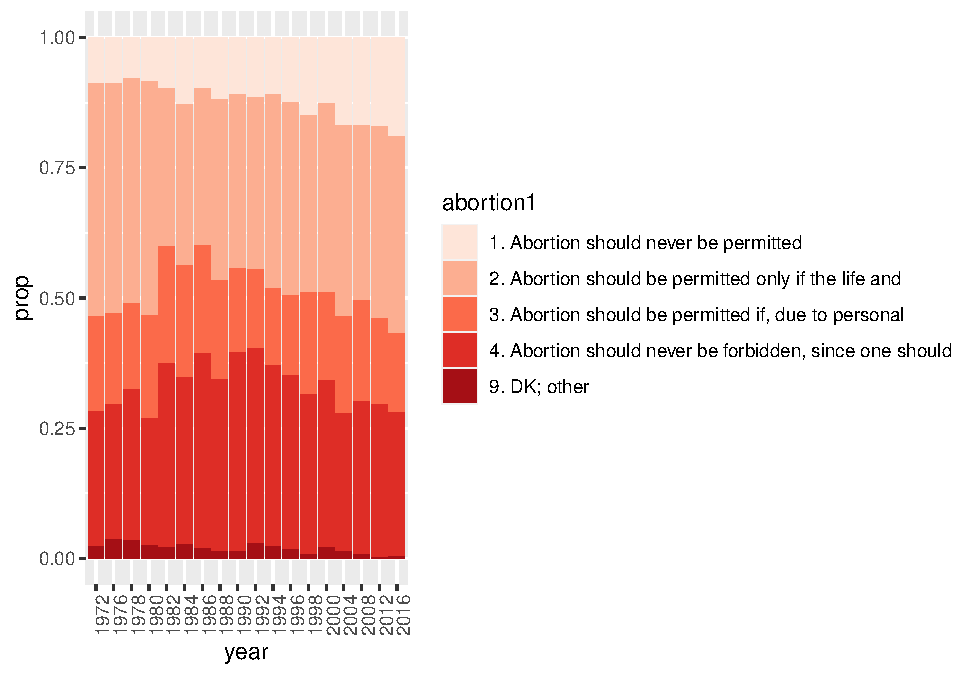
\includegraphics[width=0.5\linewidth]{Project1_NWilliams_files/figure-latex/figures-side-1}
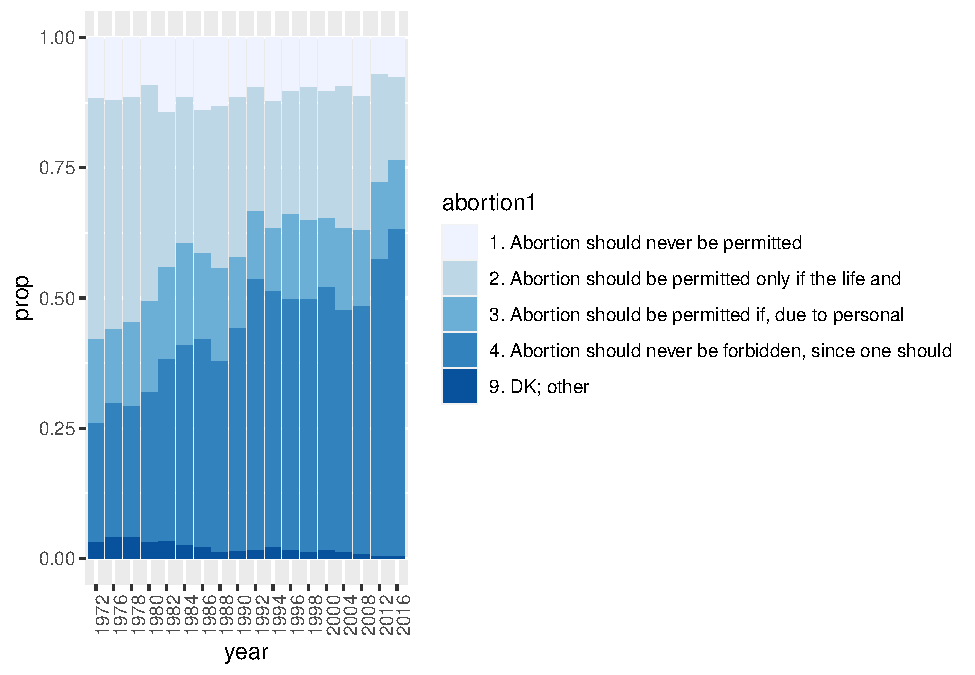
\includegraphics[width=0.5\linewidth]{Project1_NWilliams_files/figure-latex/figures-side-2}

Wow! In the first year of this question, 1972, 23\% of Democrats and
\textbf{\emph{26\%}} of Republicans answered that Abortion should never
be forbidden! Its very surprising that according to the ANES data, in
1972 a larger proportion of Republicans supported fully legal abortion
than Democrats!

However, results from 2016 are very different. While the proportion of
Republicans that answered ``Abortion should never by forbidden''
remained largely the same at 27.7\%, the amount of Democrats that
answered that way rose to a staggering 63\%!

In 1972, the largest portion of Republicans chose ``Abortion should be
permitted only if the life and health of the woman is in danger.''(45\%)
the same was true in 2016, with 37\% of Republicans answering this way.
Democrats, on the other hand, saw a shift. The most common response in
1972 was the same as Republicans: ``Abortion should be permitted only if
the life and health of the woman is in danger.''(46\%) However, unlike
Republicans, Democrats overwhelmingly chose ``Abortion should never be
forbidden'' in 2016.

So, while in 1972 Democrats and Republicans had similar views on
abortion, in 2016 the majority of Democrats believe abortion should
never be forbidden, while Republican views on abortion have only changed
slightly

\hypertarget{b-immigrants}{%
\subparagraph{1b) Immigrants}\label{b-immigrants}}

This is a thermometer question. Lower values correspond to ``Colder''
feelings. Answers that are: ``98. DK (exc. 1964-1968: see VCF0201
note)'',``99. NA; no Post IW; form III,IV (1972); breakoff,sufficient
partial (2016)'' were removed to avoid manipulating numeric
calculations.

\begin{Shaded}
\begin{Highlighting}[]
\KeywordTok{library}\NormalTok{(ggrepel)}
\KeywordTok{load}\NormalTok{(}\DataTypeTok{file=}\StringTok{"../output/all_Democrats.RData"}\NormalTok{)}
\KeywordTok{load}\NormalTok{(}\DataTypeTok{file=}\StringTok{"../output/all_Republicans.RData"}\NormalTok{)}

\StringTok{`}\DataTypeTok\StringTok{`}\NormalTok{ <-}\StringTok{ }\ControlFlowTok{function}\NormalTok{(a,b) }\OperatorTok{!}\StringTok{ }\NormalTok{a }\OperatorTok\StringTok{ }\NormalTok{b}

\CommentTok{# Democrats}
\NormalTok{demIA <-}\StringTok{ }\NormalTok{all_Democrats}\OperatorTok
\StringTok{  }\KeywordTok{select}\NormalTok{(year, illegalAliens)}\OperatorTok
\StringTok{  }\KeywordTok{filter}\NormalTok{(}\OperatorTok{!}\KeywordTok{is.na}\NormalTok{(illegalAliens))}\OperatorTok
\StringTok{  }\KeywordTok{filter}\NormalTok{(illegalAliens }\OperatorTok\StringTok{ }\KeywordTok{c}\NormalTok{(}\StringTok{"98. DK  (exc. 1964-1968: see VCF0201 note)"}\NormalTok{,}
                               \StringTok{"99. NA; no Post IW; form III,IV (1972); breakoff,   sufficient partial (2016)"}\NormalTok{))}\OperatorTok
\StringTok{  }\KeywordTok{group_by}\NormalTok{(year)}\OperatorTok
\StringTok{  }\KeywordTok{mutate}\NormalTok{(}
    \DataTypeTok{Average =} \KeywordTok{mean}\NormalTok{(}\KeywordTok{as.numeric}\NormalTok{(illegalAliens))}
\NormalTok{  )}\OperatorTok
\StringTok{  }\KeywordTok{distinct}\NormalTok{(year, }\DataTypeTok{.keep_all=}\OtherTok{TRUE}\NormalTok{)}

\CommentTok{# Republicans  }
\NormalTok{repIA <-}\StringTok{ }\NormalTok{all_Republicans}\OperatorTok
\StringTok{  }\KeywordTok{select}\NormalTok{(year, illegalAliens)}\OperatorTok
\StringTok{  }\KeywordTok{filter}\NormalTok{(}\OperatorTok{!}\KeywordTok{is.na}\NormalTok{(illegalAliens))}\OperatorTok
\StringTok{  }\KeywordTok{filter}\NormalTok{(illegalAliens }\OperatorTok\StringTok{ }\KeywordTok{c}\NormalTok{(}\StringTok{"98. DK  (exc. 1964-1968: see VCF0201 note)"}\NormalTok{,}
                               \StringTok{"99. NA; no Post IW; form III,IV (1972); breakoff,   sufficient partial (2016)"}\NormalTok{))}\OperatorTok
\StringTok{  }\KeywordTok{group_by}\NormalTok{(year)}\OperatorTok
\StringTok{  }\KeywordTok{mutate}\NormalTok{(}
    \DataTypeTok{Average =} \KeywordTok{mean}\NormalTok{(}\KeywordTok{as.numeric}\NormalTok{(illegalAliens))}
\NormalTok{  )}\OperatorTok
\StringTok{  }\KeywordTok{distinct}\NormalTok{(year, }\DataTypeTok{.keep_all=}\OtherTok{TRUE}\NormalTok{)}

\CommentTok{# Must combine the Democrate and Republican Results}
\NormalTok{IA <-}\StringTok{ }\KeywordTok{data.frame}\NormalTok{(}
\NormalTok{  demIA}\OperatorTok{$}\NormalTok{year, demIA}\OperatorTok{$}\NormalTok{Average, repIA}\OperatorTok{$}\NormalTok{Average}
\NormalTok{)}\OperatorTok
\StringTok{  }\KeywordTok{rename}\NormalTok{(}
    \DataTypeTok{Year =}\NormalTok{ demIA.year,}
    \DataTypeTok{Democrat_Average =}\NormalTok{ demIA.Average,}
    \DataTypeTok{Republican_Average =}\NormalTok{ repIA.Average}
\NormalTok{  )}\OperatorTok
\StringTok{  }\KeywordTok{mutate}\NormalTok{(}
    \DataTypeTok{Percent_Difference =} \DecValTok{2}\OperatorTok{*}\NormalTok{(Democrat_Average }\OperatorTok{-}\StringTok{ }\NormalTok{Republican_Average)}\OperatorTok{/}\NormalTok{(Democrat_Average}\OperatorTok{+}\NormalTok{Republican_Average)  }
\NormalTok{    )}


\CommentTok{# This Pipe is solely to obtain labels for the beginning and end points. }
\NormalTok{IAplot <-}\StringTok{ }\NormalTok{IA}\OperatorTok
\StringTok{  }\KeywordTok{mutate}\NormalTok{(}
    \DataTypeTok{labelDem1 =}\KeywordTok{if_else}\NormalTok{(Year}\OperatorTok{==}\KeywordTok{first}\NormalTok{(IA}\OperatorTok{$}\NormalTok{Year),}
                      \DataTypeTok{true =} \KeywordTok{as.character}\NormalTok{(}\KeywordTok{round}\NormalTok{(}\KeywordTok{first}\NormalTok{(IA}\OperatorTok{$}\NormalTok{Democrat_Average), }\DataTypeTok{digits =} \DecValTok{1}\NormalTok{)),}
                      \DataTypeTok{false=} \StringTok{""}
\NormalTok{    ),}
    \DataTypeTok{labelDem2 =}\KeywordTok{if_else}\NormalTok{(Year}\OperatorTok{==}\KeywordTok{last}\NormalTok{(IA}\OperatorTok{$}\NormalTok{Year),}
                      \DataTypeTok{true =} \KeywordTok{as.character}\NormalTok{(}\KeywordTok{round}\NormalTok{(}\KeywordTok{last}\NormalTok{(IA}\OperatorTok{$}\NormalTok{Democrat_Average), }\DataTypeTok{digits =} \DecValTok{1}\NormalTok{)),}
                      \DataTypeTok{false=} \StringTok{""}
\NormalTok{    ),}
    \DataTypeTok{labelRep1 =}\KeywordTok{if_else}\NormalTok{(Year}\OperatorTok{==}\KeywordTok{first}\NormalTok{(IA}\OperatorTok{$}\NormalTok{Year),}
                      \DataTypeTok{true =} \KeywordTok{as.character}\NormalTok{(}\KeywordTok{round}\NormalTok{(}\KeywordTok{first}\NormalTok{(IA}\OperatorTok{$}\NormalTok{Republican_Average), }\DataTypeTok{digits =} \DecValTok{1}\NormalTok{)),}
                      \DataTypeTok{false=} \StringTok{""}
\NormalTok{    ),}
    \DataTypeTok{labelRep2 =}\KeywordTok{if_else}\NormalTok{(Year}\OperatorTok{==}\KeywordTok{last}\NormalTok{(IA}\OperatorTok{$}\NormalTok{Year),}
                      \DataTypeTok{true =} \KeywordTok{as.character}\NormalTok{(}\KeywordTok{round}\NormalTok{(}\KeywordTok{last}\NormalTok{(IA}\OperatorTok{$}\NormalTok{Republican_Average), }\DataTypeTok{digits =} \DecValTok{1}\NormalTok{)),}
                      \DataTypeTok{false=} \StringTok{""}
\NormalTok{    )}
\NormalTok{  )}\OperatorTok
\StringTok{  }\KeywordTok{ggplot}\NormalTok{()}\OperatorTok{+}
\StringTok{  }\KeywordTok{geom_line}\NormalTok{(}\KeywordTok{aes}\NormalTok{(}\DataTypeTok{x=}\NormalTok{ Year, }\DataTypeTok{y=}\NormalTok{ Democrat_Average, }\DataTypeTok{group=}\DecValTok{1}\NormalTok{, }\DataTypeTok{color=}\StringTok{"Democrat"}\NormalTok{))}\OperatorTok{+}
\StringTok{  }\KeywordTok{geom_line}\NormalTok{(}\KeywordTok{aes}\NormalTok{(}\DataTypeTok{x=}\NormalTok{ Year, }\DataTypeTok{y=}\NormalTok{ Republican_Average, }\DataTypeTok{group=}\DecValTok{2}\NormalTok{, }\DataTypeTok{color=}\StringTok{"Republican"}\NormalTok{))}\OperatorTok{+}
\StringTok{  }\KeywordTok{geom_label_repel}\NormalTok{(}\KeywordTok{aes}\NormalTok{(}\DataTypeTok{label=}\NormalTok{labelDem1, }\DataTypeTok{x =}\NormalTok{ Year, }\DataTypeTok{y=}\NormalTok{Democrat_Average),}\DataTypeTok{nudge_y =}\DecValTok{1}\NormalTok{)}\OperatorTok{+}
\StringTok{  }\KeywordTok{geom_label_repel}\NormalTok{(}\KeywordTok{aes}\NormalTok{(}\DataTypeTok{label=}\NormalTok{labelDem2, }\DataTypeTok{x =}\NormalTok{ Year, }\DataTypeTok{y=}\NormalTok{Democrat_Average),}\DataTypeTok{nudge_y =}\DecValTok{1}\NormalTok{)}\OperatorTok{+}
\StringTok{  }\KeywordTok{geom_label_repel}\NormalTok{(}\KeywordTok{aes}\NormalTok{(}\DataTypeTok{label=}\NormalTok{labelRep2, }\DataTypeTok{x =}\NormalTok{ Year, }\DataTypeTok{y=}\NormalTok{Republican_Average))}\OperatorTok{+}
\StringTok{  }\KeywordTok{geom_label_repel}\NormalTok{(}\KeywordTok{aes}\NormalTok{(}\DataTypeTok{label=}\NormalTok{labelRep1, }\DataTypeTok{x =}\NormalTok{ Year, }\DataTypeTok{y=}\NormalTok{Republican_Average), }\DataTypeTok{nudge_y =} \DecValTok{-1}\NormalTok{)}\OperatorTok{+}
\StringTok{  }\KeywordTok{geom_ribbon}\NormalTok{(}\KeywordTok{aes}\NormalTok{(}\DataTypeTok{x=}\NormalTok{Year, }\DataTypeTok{ymin=}\NormalTok{ Republican_Average, }\DataTypeTok{ymax=}\NormalTok{ Democrat_Average, }\DataTypeTok{group=}\DecValTok{1}\NormalTok{), }\DataTypeTok{show.legend=} \OtherTok{FALSE}\NormalTok{, }\DataTypeTok{alpha=}\FloatTok{0.5}\NormalTok{)}\OperatorTok{+}
\StringTok{  }\KeywordTok{scale_color_manual}\NormalTok{(}\DataTypeTok{values=} \KeywordTok{c}\NormalTok{(}
    \StringTok{"Democrat"}\NormalTok{ =}\StringTok{ "darkblue"}\NormalTok{, }
    \StringTok{"Republican"}\NormalTok{=}\StringTok{"red"}
\NormalTok{  ))}\OperatorTok{+}
\StringTok{  }\KeywordTok{ylab}\NormalTok{(}\StringTok{"Average Warmness Towards Illegal Aliens/ Immigrants"}\NormalTok{)}\OperatorTok{+}
\StringTok{  }\KeywordTok{ylim}\NormalTok{(}\DecValTok{0}\NormalTok{,}\DecValTok{100}\NormalTok{)}\OperatorTok{+}
\StringTok{  }\KeywordTok{xlab}\NormalTok{(}\StringTok{"Year"}\NormalTok{)}\OperatorTok{+}
\StringTok{  }\KeywordTok{labs}\NormalTok{(}\DataTypeTok{title=} \StringTok{"Warmness Towards Illegal Immigrants By Party from 1988-2016"}\NormalTok{, }\DataTypeTok{color=} \StringTok{"Party"}\NormalTok{)}

\KeywordTok{ggsave}\NormalTok{(}\DataTypeTok{path=}\StringTok{"../figs"}\NormalTok{, }\DataTypeTok{filename=}\StringTok{"illegalAlienPlot.png"}\NormalTok{)  }
\end{Highlighting}
\end{Shaded}

\begin{verbatim}
## Saving 6.5 x 4.5 in image
\end{verbatim}

\begin{Shaded}
\begin{Highlighting}[]
\KeywordTok{print}\NormalTok{(IAplot)}
\end{Highlighting}
\end{Shaded}

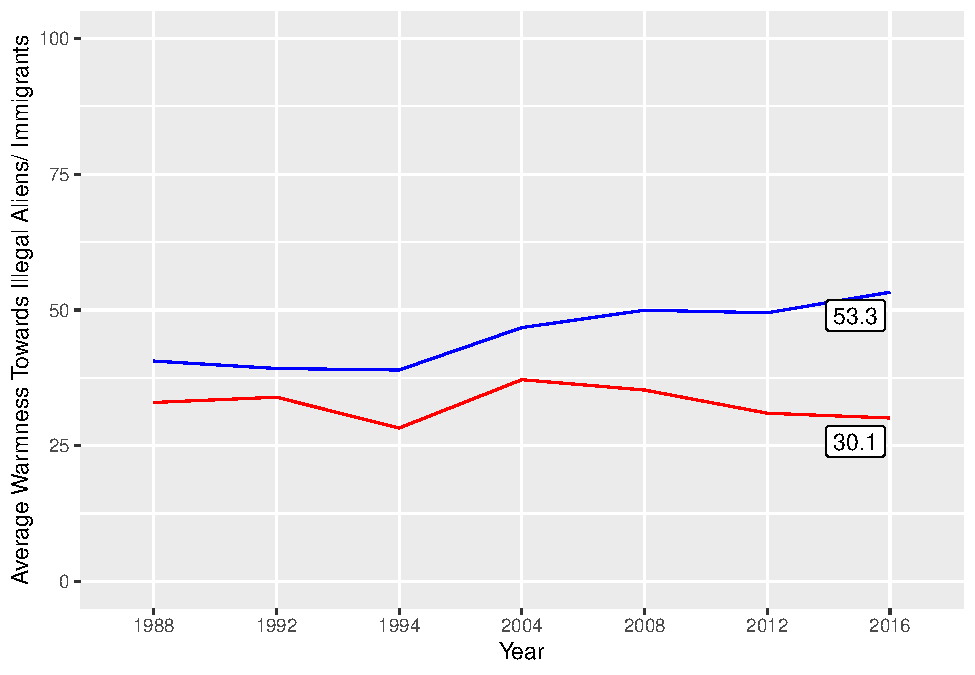
\includegraphics[width=0.5\linewidth]{Project1_NWilliams_files/figure-latex/unnamed-chunk-4-1}
This figure, clearly shows the divergence between Republicans and
Democrats over time on their feelings towards Illegal Aliens/Immigrants.
Republican Respondents attitudes only shift downwards 8.8\% indicating
that their feelings towards illegal immigrants has worsened over time.
Democrats, alternatively, see a more dramatic increase in warmness
towards Illegal Immigrants, seeing a 31.3\% increase.

\hypertarget{c-the-role-of-government-in-healthcare}{%
\subparagraph{1c) The Role of Government in
Healthcare?}\label{c-the-role-of-government-in-healthcare}}

\begin{Shaded}
\begin{Highlighting}[]
\KeywordTok{load}\NormalTok{(}\DataTypeTok{file=}\StringTok{"../output/all_Democrats.RData"}\NormalTok{)}
\KeywordTok{load}\NormalTok{(}\DataTypeTok{file=}\StringTok{"../output/all_Republicans.RData"}\NormalTok{)}

\CommentTok{# Democrats and Healthcare}
\CommentTok{# Two questions but  with different answers use question healthcare2 }
\StringTok{`}\DataTypeTok\StringTok{`}\NormalTok{ <-}\StringTok{ }\ControlFlowTok{function}\NormalTok{(a,b) }\OperatorTok{!}\StringTok{ }\NormalTok{a }\OperatorTok\StringTok{ }\NormalTok{b}

\NormalTok{demHC <-}\StringTok{ }\NormalTok{all_Democrats}\OperatorTok
\StringTok{  }\KeywordTok{select}\NormalTok{(year, healthcare2)}\OperatorTok
\StringTok{  }\KeywordTok{filter}\NormalTok{(}\OperatorTok{!}\KeywordTok{is.na}\NormalTok{(healthcare2))}\OperatorTok
\StringTok{  }\KeywordTok{filter}\NormalTok{(healthcare2 }\OperatorTok\StringTok{ }\KeywordTok{c}\NormalTok{(}\StringTok{"9. DK; haven't thought much about it"}\NormalTok{))}
  

\NormalTok{repHC <-}\StringTok{ }\NormalTok{all_Republicans}\OperatorTok
\StringTok{  }\KeywordTok{select}\NormalTok{(year, healthcare2)}\OperatorTok
\StringTok{  }\KeywordTok{filter}\NormalTok{(}\OperatorTok{!}\KeywordTok{is.na}\NormalTok{(healthcare2))}\OperatorTok
\StringTok{  }\KeywordTok{filter}\NormalTok{(healthcare2 }\OperatorTok\StringTok{ }\KeywordTok{c}\NormalTok{(}\StringTok{"9. DK; haven't thought much about it"}\NormalTok{))}

\KeywordTok{save}\NormalTok{(repHC, }\DataTypeTok{file=}\StringTok{"../output/republicans_HealthCare.RData"}\NormalTok{)}
\KeywordTok{save}\NormalTok{(demHC, }\DataTypeTok{file=}\StringTok{"../output/democrats_HealthCare.RData"}\NormalTok{)}
\end{Highlighting}
\end{Shaded}

How have Democrats and Republicans Views on Healthcare Changed Over
Time?

Another Spectrum Question ``1'' \textless- There should be a
Nationalized Health Care Service, to ``7'' \textless- Entirely Private
Insurance Plans. ``9'' \textless-9. DK; haven't thought much about it

\begin{Shaded}
\begin{Highlighting}[]
\KeywordTok{load}\NormalTok{(}\DataTypeTok{file=}\StringTok{"../output/democrats_HealthCare.Rdata"}\NormalTok{)}
\KeywordTok{load}\NormalTok{(}\DataTypeTok{file=}\StringTok{"../output/republicans_HealthCare.RData"}\NormalTok{)}

\NormalTok{demHC_df <-}\StringTok{ }\NormalTok{demHC }\OperatorTok
\StringTok{  }\KeywordTok{group_by}\NormalTok{(year, healthcare2)}\OperatorTok
\StringTok{  }\KeywordTok{summarize}\NormalTok{(}\DataTypeTok{n=}\KeywordTok{n}\NormalTok{())}\OperatorTok
\StringTok{  }\KeywordTok{mutate}\NormalTok{(}
    \DataTypeTok{prop=}\NormalTok{n}\OperatorTok{/}\KeywordTok{sum}\NormalTok{(n)}
\NormalTok{  )}
\end{Highlighting}
\end{Shaded}

\begin{verbatim}
## `summarise()` regrouping output by 'year' (override with `.groups` argument)
\end{verbatim}

\begin{Shaded}
\begin{Highlighting}[]
\NormalTok{repHC_df <-}\StringTok{ }\NormalTok{repHC }\OperatorTok
\StringTok{  }\KeywordTok{group_by}\NormalTok{(year, healthcare2)}\OperatorTok
\StringTok{  }\KeywordTok{summarize}\NormalTok{(}\DataTypeTok{n=}\KeywordTok{n}\NormalTok{())}\OperatorTok
\StringTok{  }\KeywordTok{mutate}\NormalTok{(}
    \DataTypeTok{prop=}\NormalTok{n}\OperatorTok{/}\KeywordTok{sum}\NormalTok{(n)}
\NormalTok{  )}
\end{Highlighting}
\end{Shaded}

\begin{verbatim}
## `summarise()` regrouping output by 'year' (override with `.groups` argument)
\end{verbatim}

\begin{Shaded}
\begin{Highlighting}[]
\KeywordTok{ggplot}\NormalTok{(repHC_df, }\KeywordTok{aes}\NormalTok{(}\DataTypeTok{x=}\NormalTok{year, }\DataTypeTok{y=}\NormalTok{prop, }\DataTypeTok{fill=}\NormalTok{healthcare2))}\OperatorTok{+}
\StringTok{  }\KeywordTok{geom_bar}\NormalTok{(}\DataTypeTok{stat =} \StringTok{"identity"}\NormalTok{)}\OperatorTok{+}
\StringTok{  }\KeywordTok{theme}\NormalTok{(}\DataTypeTok{axis.text.x =} \KeywordTok{element_text}\NormalTok{(}\DataTypeTok{angle =} \DecValTok{90}\NormalTok{))}\OperatorTok{+}
\StringTok{  }\KeywordTok{scale_fill_brewer}\NormalTok{(}\DataTypeTok{palette =} \StringTok{"Reds"}\NormalTok{)}

\KeywordTok{ggplot}\NormalTok{(demHC_df, }\KeywordTok{aes}\NormalTok{(}\DataTypeTok{x=}\NormalTok{year, }\DataTypeTok{y=}\NormalTok{prop, }\DataTypeTok{fill=}\NormalTok{healthcare2))}\OperatorTok{+}
\StringTok{  }\KeywordTok{geom_bar}\NormalTok{(}\DataTypeTok{stat =} \StringTok{"identity"}\NormalTok{)}\OperatorTok{+}
\StringTok{  }\KeywordTok{theme}\NormalTok{(}\DataTypeTok{axis.text.x =} \KeywordTok{element_text}\NormalTok{(}\DataTypeTok{angle =} \DecValTok{90}\NormalTok{))}\OperatorTok{+}
\StringTok{  }\KeywordTok{scale_fill_brewer}\NormalTok{(}\DataTypeTok{palette =} \StringTok{"Blues"}\NormalTok{)}
\end{Highlighting}
\end{Shaded}

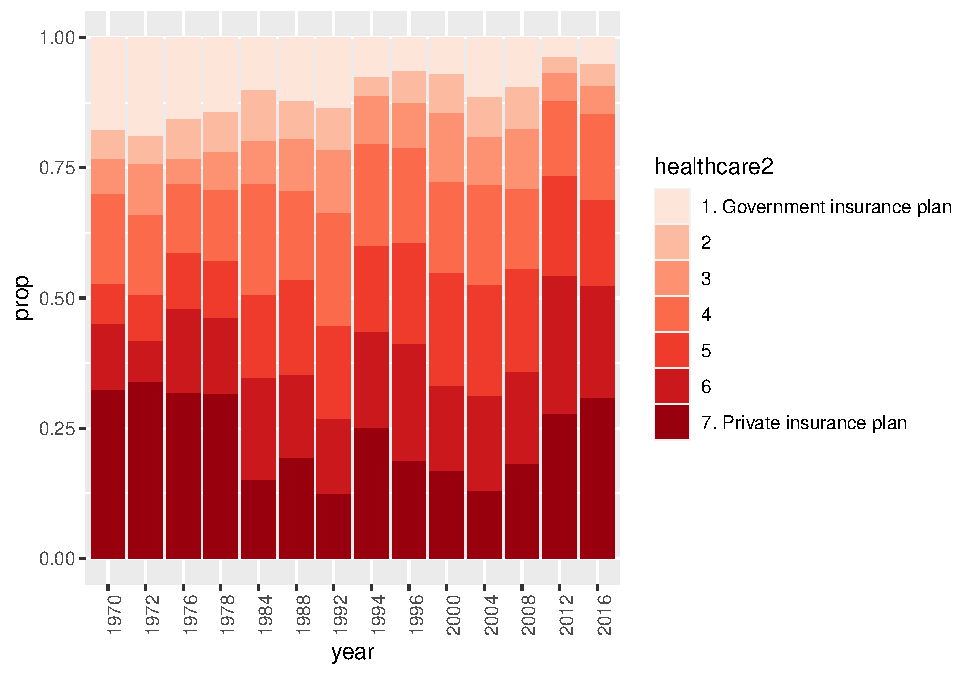
\includegraphics[width=0.5\linewidth]{Project1_NWilliams_files/figure-latex/unnamed-chunk-6-1}
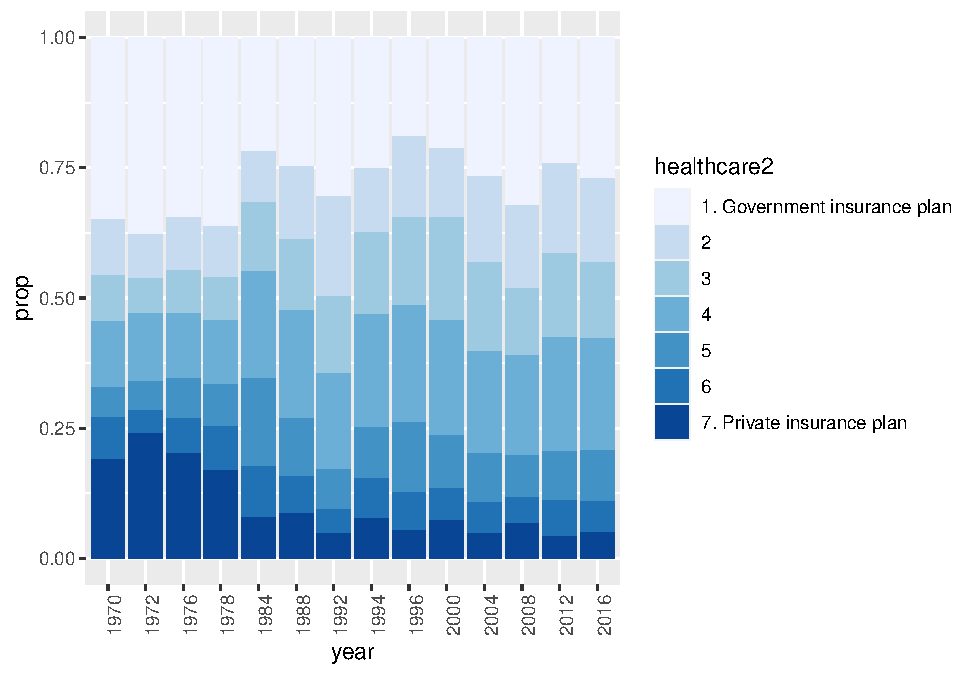
\includegraphics[width=0.5\linewidth]{Project1_NWilliams_files/figure-latex/unnamed-chunk-6-2}
The results of this question are unique in that substantial differences
are seen even in the first year of the question, 1970. In 1970, 32.3\%
of Republicans felt that private insurance insurances should make up the
entirety of health insurance. While only 18\% of democrats felt the same
way.

Democrat's most common answer in 1970 was surprisingly, ``1. Government
Insurance Plan'', with 34.9\% of the respondents.

So even in 1970, surveyed Democrats and Republicans felt very different
about this. How about in 2016? In 2016, the proportion of Republicans
who answered ``1. Government Insurance Plan'' dropped from 17.8\% to
only 5.3\%.

Also interesting, the proportion of Democrats who answered in favor of
fully nationalized healthcare (Option:``1. Government Insurance Plan'')
decreased to 27.1\%.

So Republicans and Democrats since 1970 have had very different views on
the role of Government in Healthcare, but since 1970 their views have
largely not diverged greater.

\hypertarget{d-another-issue-the-military}{%
\subparagraph{1d) Another issue: The
military}\label{d-another-issue-the-military}}

Spectrum: ``1'' \textless- Greatly Decrease defense Spending, ``7''
\textless- Greatly Increase defense Spending ``9'' \textless-9. DK;
haven't thought much about it

\begin{Shaded}
\begin{Highlighting}[]
\CommentTok{# Military Analysis}
\KeywordTok{load}\NormalTok{(}\DataTypeTok{file=}\StringTok{"../output/all_Democrats.RData"}\NormalTok{)}
\KeywordTok{load}\NormalTok{(}\DataTypeTok{file=}\StringTok{"../output/all_Republicans.RData"}\NormalTok{)}

\NormalTok{militaryDem <-}\StringTok{ }\NormalTok{all_Democrats}\OperatorTok
\StringTok{  }\KeywordTok{select}\NormalTok{(year, militarySpending2)}\OperatorTok
\StringTok{  }\KeywordTok{filter}\NormalTok{(}\OperatorTok{!}\KeywordTok{is.na}\NormalTok{(militarySpending2))}\OperatorTok
\StringTok{  }\KeywordTok{group_by}\NormalTok{(year, militarySpending2)}\OperatorTok
\StringTok{  }\KeywordTok{summarize}\NormalTok{(}\DataTypeTok{n=}\KeywordTok{n}\NormalTok{())}\OperatorTok
\StringTok{  }\KeywordTok{mutate}\NormalTok{(}
    \DataTypeTok{prop=}\NormalTok{n}\OperatorTok{/}\KeywordTok{sum}\NormalTok{(n)}
\NormalTok{  )}
\end{Highlighting}
\end{Shaded}

\begin{verbatim}
## `summarise()` regrouping output by 'year' (override with `.groups` argument)
\end{verbatim}

\begin{Shaded}
\begin{Highlighting}[]
\NormalTok{militaryRep <-}\StringTok{ }\NormalTok{all_Republicans}\OperatorTok
\StringTok{  }\KeywordTok{select}\NormalTok{(year, militarySpending2)}\OperatorTok
\StringTok{  }\KeywordTok{filter}\NormalTok{(}\OperatorTok{!}\KeywordTok{is.na}\NormalTok{(militarySpending2))}\OperatorTok
\StringTok{  }\KeywordTok{group_by}\NormalTok{(year, militarySpending2)}\OperatorTok
\StringTok{  }\KeywordTok{summarize}\NormalTok{(}\DataTypeTok{n=}\KeywordTok{n}\NormalTok{())}\OperatorTok
\StringTok{  }\KeywordTok{mutate}\NormalTok{(}
    \DataTypeTok{prop=}\NormalTok{n}\OperatorTok{/}\KeywordTok{sum}\NormalTok{(n)}
\NormalTok{  )}
\end{Highlighting}
\end{Shaded}

\begin{verbatim}
## `summarise()` regrouping output by 'year' (override with `.groups` argument)
\end{verbatim}

\begin{Shaded}
\begin{Highlighting}[]
\KeywordTok{ggplot}\NormalTok{(militaryRep, }\KeywordTok{aes}\NormalTok{(}\DataTypeTok{x=}\NormalTok{year, }\DataTypeTok{y=}\NormalTok{prop, }\DataTypeTok{fill=}\NormalTok{militarySpending2))}\OperatorTok{+}
\StringTok{  }\KeywordTok{geom_bar}\NormalTok{(}\DataTypeTok{stat =} \StringTok{"identity"}\NormalTok{)}\OperatorTok{+}
\StringTok{  }\KeywordTok{theme}\NormalTok{(}\DataTypeTok{axis.text.x =} \KeywordTok{element_text}\NormalTok{(}\DataTypeTok{angle =} \DecValTok{90}\NormalTok{))}\OperatorTok{+}
\StringTok{  }\KeywordTok{scale_fill_brewer}\NormalTok{(}\DataTypeTok{palette =} \StringTok{"Reds"}\NormalTok{)}

\KeywordTok{ggplot}\NormalTok{(militaryDem, }\KeywordTok{aes}\NormalTok{(}\DataTypeTok{x=}\NormalTok{year, }\DataTypeTok{y=}\NormalTok{prop, }\DataTypeTok{fill=}\NormalTok{militarySpending2))}\OperatorTok{+}
\StringTok{  }\KeywordTok{geom_bar}\NormalTok{(}\DataTypeTok{stat =} \StringTok{"identity"}\NormalTok{)}\OperatorTok{+}
\StringTok{  }\KeywordTok{theme}\NormalTok{(}\DataTypeTok{axis.text.x =} \KeywordTok{element_text}\NormalTok{(}\DataTypeTok{angle =} \DecValTok{90}\NormalTok{))}\OperatorTok{+}
\StringTok{  }\KeywordTok{scale_fill_brewer}\NormalTok{(}\DataTypeTok{palette =} \StringTok{"Blues"}\NormalTok{)}
\end{Highlighting}
\end{Shaded}

\includegraphics[width=0.5\linewidth]{Project1_NWilliams_files/figure-latex/unnamed-chunk-7-1}
\includegraphics[width=0.5\linewidth]{Project1_NWilliams_files/figure-latex/unnamed-chunk-7-2}
This question is interesting because it does not focus on domestic
issues. Since the recent Iraq War and the war in Afghanistan, did not
take place on American soil, ideas surrounding the military can be more
abstract to the American populace. This is supported by 14\% of
Democratic respondents who answered ``DK; haven't thought much about
it'' (2016).

The topic of military spending is the least polarizing issue in this
analysis. In 1980, Democrats and Republicans most commonly answered
``5'', and ``6'' respectively on the scale of 1-7. In 2016, the most
common answer for Democrats and Republicans was ``4'', and ``5''
respectively again.

\hypertarget{e-lastly-government-aid-for-minorities}{%
\subparagraph{1e) Lastly: Government Aid for
Minorities}\label{e-lastly-government-aid-for-minorities}}

Spectrum: ``1'' Government should help minority groups/blacks , ``7''
\textless- Minority groups/ blacks should help themselves, ``9''
\textless-9. DK; haven't thought much about it

\begin{Shaded}
\begin{Highlighting}[]
\KeywordTok{load}\NormalTok{(}\DataTypeTok{file=}\StringTok{"../output/data_use.RData"}\NormalTok{)}

\StringTok{`}\DataTypeTok\StringTok{`}\NormalTok{ <-}\StringTok{ }\ControlFlowTok{function}\NormalTok{(a,b) }\OperatorTok{!}\StringTok{ }\NormalTok{a }\OperatorTok\StringTok{ }\NormalTok{b}

\NormalTok{govHelpAll <-}\StringTok{ }\NormalTok{anes_use}\OperatorTok
\StringTok{  }\KeywordTok{select}\NormalTok{(year, party_scale, govHelp)}\OperatorTok
\StringTok{  }\KeywordTok{filter}\NormalTok{(}\OperatorTok{!}\KeywordTok{is.na}\NormalTok{(party_scale)}\OperatorTok{&}\StringTok{ }\OperatorTok{!}\KeywordTok{is.na}\NormalTok{(govHelp))}\OperatorTok
\StringTok{  }\KeywordTok{filter}\NormalTok{(govHelp }\OperatorTok\StringTok{ }\KeywordTok{c}\NormalTok{(}\StringTok{"9. DK; haven't thought much about it"}\NormalTok{))}\OperatorTok
\StringTok{   }\KeywordTok{group_by}\NormalTok{(year, party_scale)}\OperatorTok
\StringTok{  }\KeywordTok{count}\NormalTok{(govHelp)}\OperatorTok
\StringTok{  }\KeywordTok{group_by}\NormalTok{(year, party_scale)}\OperatorTok
\StringTok{  }\KeywordTok{mutate}\NormalTok{(}
    \DataTypeTok{Percent =} \DecValTok{100} \OperatorTok{*}\StringTok{ }\NormalTok{(n}\OperatorTok{/}\StringTok{ }\KeywordTok{sum}\NormalTok{(n))}
\NormalTok{  )}
\KeywordTok{save}\NormalTok{(govHelpAll, }\DataTypeTok{file=}\StringTok{"../output/all_govHelp.RData"}\NormalTok{)}
\end{Highlighting}
\end{Shaded}

\begin{Shaded}
\begin{Highlighting}[]
\KeywordTok{load}\NormalTok{(}\DataTypeTok{file=}\StringTok{"../output/all_govHelp.RData"}\NormalTok{)}

\NormalTok{years <-}\StringTok{ }\KeywordTok{c}\NormalTok{(}\StringTok{"1970"}\NormalTok{,}\StringTok{"1980"}\NormalTok{,}\StringTok{"1990"}\NormalTok{,}\StringTok{"2000"}\NormalTok{,}\StringTok{"2010"}\NormalTok{,}\StringTok{"2016"}\NormalTok{)}

\CommentTok{# "Poles" are the furtherest respondents of each party, Strong Democrats and Strong Republicans. }

\NormalTok{poles<-}\StringTok{ }\NormalTok{govHelpAll}\OperatorTok
\StringTok{  }\KeywordTok{select}\NormalTok{(year, party_scale, govHelp, Percent)}\OperatorTok
\StringTok{  }\KeywordTok{filter}\NormalTok{(}\KeywordTok{as.character}\NormalTok{(party_scale)}\OperatorTok\StringTok{ }\KeywordTok{c}\NormalTok{(}\StringTok{"1. Strong Democrat"}\NormalTok{,}\StringTok{"7. Strong Republican"}\NormalTok{))}\OperatorTok
\StringTok{  }\KeywordTok{filter}\NormalTok{(}\KeywordTok{as.character}\NormalTok{(year) }\OperatorTok\StringTok{ }\NormalTok{years)}\OperatorTok
\StringTok{  }\KeywordTok{group_by}\NormalTok{(govHelp, year)}

\KeywordTok{ggplot}\NormalTok{(poles, }\KeywordTok{aes}\NormalTok{(govHelp, Percent, }\DataTypeTok{fill=}\NormalTok{party_scale))}\OperatorTok{+}
\StringTok{  }\KeywordTok{geom_bar}\NormalTok{(}\DataTypeTok{stat =} \StringTok{"identity"}\NormalTok{, }\DataTypeTok{position=}\StringTok{"dodge"}\NormalTok{)}\OperatorTok{+}
\StringTok{  }\KeywordTok{facet_wrap}\NormalTok{(}\OperatorTok{~}\NormalTok{year, }\DataTypeTok{ncol =} \DecValTok{1}\NormalTok{)}\OperatorTok{+}
\StringTok{  }\KeywordTok{scale_fill_manual}\NormalTok{(}\DataTypeTok{values=}\KeywordTok{c}\NormalTok{(}\StringTok{"blue"}\NormalTok{, }\StringTok{"red"}\NormalTok{))}\OperatorTok{+}
\StringTok{  }\KeywordTok{labs}\NormalTok{(}\DataTypeTok{title=}\StringTok{"How Did Strong Democrats & Republicans Feel About Government}\CharTok{\textbackslash{}n}\StringTok{for Minorities over the years?"}\NormalTok{)}
\end{Highlighting}
\end{Shaded}

\includegraphics{Project1_NWilliams_files/figure-latex/unnamed-chunk-9-1.pdf}
In this question, we see a similar pattern that was since with Democrats
and how they felt about abortion. Over time, Democrats felt more and
more strongly that abortion should never be forbidden. Republicans did
become more conservative as well, but much slower then Democrats became
more liberal and polar in their view.

This phenomenon occured again, but this time, Republicans were the party
that became much more steadfast in their opinion on the question at
hand. As we can see in the above figure, in 1970, 22.5\% of Republicans
felt that ``7. Minority groups/blacks should help themselves'', while
this is still a substantial proportion of respondents, in 2016, this
proportion nearly doubles to \textbf{39\%!}. After 2000, the proportion
of Republicans who feel exactly in the middle between ``1. The
Government should help minority groups/blacks'' and ``7. Minority
groups/blacks should help themselves'' decreased, and respondents
increasingly answered more towards 7.

While Republicans' responses are changing, Democrats are remaining
nearly constant. In 1970, 24\% of respondents answered ``4'' so right in
the middle of the spectrum. In 2016, this remained nearly the same with
25\% of respondents answering that way.

\hypertarget{iv.-discussion}{%
\subsubsection{\texorpdfstring{\textbf{IV. Discussion
}}{IV. Discussion }}\label{iv.-discussion}}

From the five issues investigated here, three conclusions can be drawn
about political polarization in America. -1) Republicans and Democrats
are more likely to have diverging views on social issues, as opposed to
foreign affairs.

This conclusion is drawn from results on Military Spending. Democrats
and Republicans views on Military Spending do not vary much over time,
and do not show major differences across parties. Respondents mostly
placed themselves on the middle of the spectrum ( with Republicans
mostly answering ``5'' and Democrats ``4''), and this did not largely
change from 1980 to 2016. One cause of this is that Americans are not
``face to face'' with military spending in their daily lives, and thus
are less informed and/or more apathetic about the issue.

-2) Democrats and Republicans views on social issues ARE very polar, but
this isn't a new phenomenon.

This conclusion somewhat counteracts the current hype that American
politics have never been more polarizing then they are right now.
Although there is polarization between Democrats and Republicans, the
data reflected from ANES shows that in the 1970 and 1980's there was
polarization. This is best supported by the results of ``Government Aid
for Minorities'' and ``Healthcare''. In the 1970, Democrats and
Republicans felt very differently about the role of goverment in health
care. While 34\% of Democrats supported a Government insurance plan,
only 14\% of Republicans were in favor (1970). In 2016, the difference
had widened, with 27\% of democrats and 5\% of Republicans supporting a
Government insurance plan but it hadn't appeared out of the blue.

-3) Certain issues polarization certain parties more.

Democrats' attitudes towards illegal Immigrants warmed significantly,
increasing by 31\%. Republican's attitudes towards illegal Immigrants
did sour, but not as drastically as Democrats warmed.

Further, Democrats views on abortion became increasingly polarized while
Republicans views did as well, but at a much slower rate. In 1972, only
23\% of Democrats answered that abortion should never by forbidden, and
in 2016 this proportion rose to 63\%. Whereas, in 1972, 26\% of
Republicans answered that abortion should never be forbidden and this
number remained nearly the same in 2016, 27\%.

\hypertarget{v.-limitations-and-recommendations}{%
\subsubsection{\texorpdfstring{\textbf{V. Limitations and
Recommendations
}}{V. Limitations and Recommendations }}\label{v.-limitations-and-recommendations}}

This analysis is limited in that the respondents may not represent the
American populace well. Respondents were paid on a sliding scale for how
much of the survey they completed. This may yield data of low quality:
answering randomly, not reading questions before answering etc. Future
studies could focus on the confidence level of the data.

Another limitation of this analysis is depth. The analysis of government
aid for minorities only reflected respondents that called themselves
``Strong'' Democrats or Republicans. A deeper analysis could compare how
other `strengths' of Democrat and Republican respondents feel about
government aid.

Finally, this analysis could be enhanced in future studies by comparing
changes within the Democratic and Republican Parties over time, i.e.~has
the proportion of Democrats who describe themselves as ``Strong
Democrats'' increased or decreased.

\end{document}
